\section{Results on the NEPSE Universe}
\label{sec:results}

\subsection{Headline Network Statistics}
\label{sec:results-headline}

We now report results on the full NEPSE panel (\emph{max} window,
$T=\num{5796}$ days, $N=372$ stocks, $k=5$).  The top-$5$ sparsified
graph contains $\num{1549}$ edges (density
$\rho_{\text{edge}}=2|E|/(N(N-1))=\num{0.0225}$); we extract its
Minimum Spanning Tree for visualisation, which contains $N-1=371$
edges and has the canonical density
$\rho_{\text{edge}}=2/(N)\approx\SI{0.5}{\percent}$.  Louvain on the
top-$5$ graph detects $n_c=7$ communities with modularity
$Q=0.6609$ (mean $\pm$ std over ten seeds).  The 11
community sizes, ranked, are
$\{54, 47, 45, 42, 38, 36, 34, 28, 22, 14, 12\}$ (median $38$, largest
share \SI{14.5}{\percent}).

\subsection{Sector--Community Alignment}
\label{sec:results-alignment}

We measure the alignment between the detected communities and the
official sector map using the \emph{adjusted Rand index}
(ARI)~\cite{hubert1985part}.  The full universe yields $\text{ARI}=0.21$
(informative: a pure random partition would yield $\text{ARI}\approx 0$
and a perfect match $\text{ARI}=1$).  This is consistent with the
international literature~\cite{brida2010dynamical, podosu2013network}:
the correlation network does \emph{not} reproduce the official sector
taxonomy, but it is \emph{not} independent of it either.  The detected
communities are a re-arrangement that picks up shared factor exposures
not captured by sector.

\begin{figure}[H]
\centering
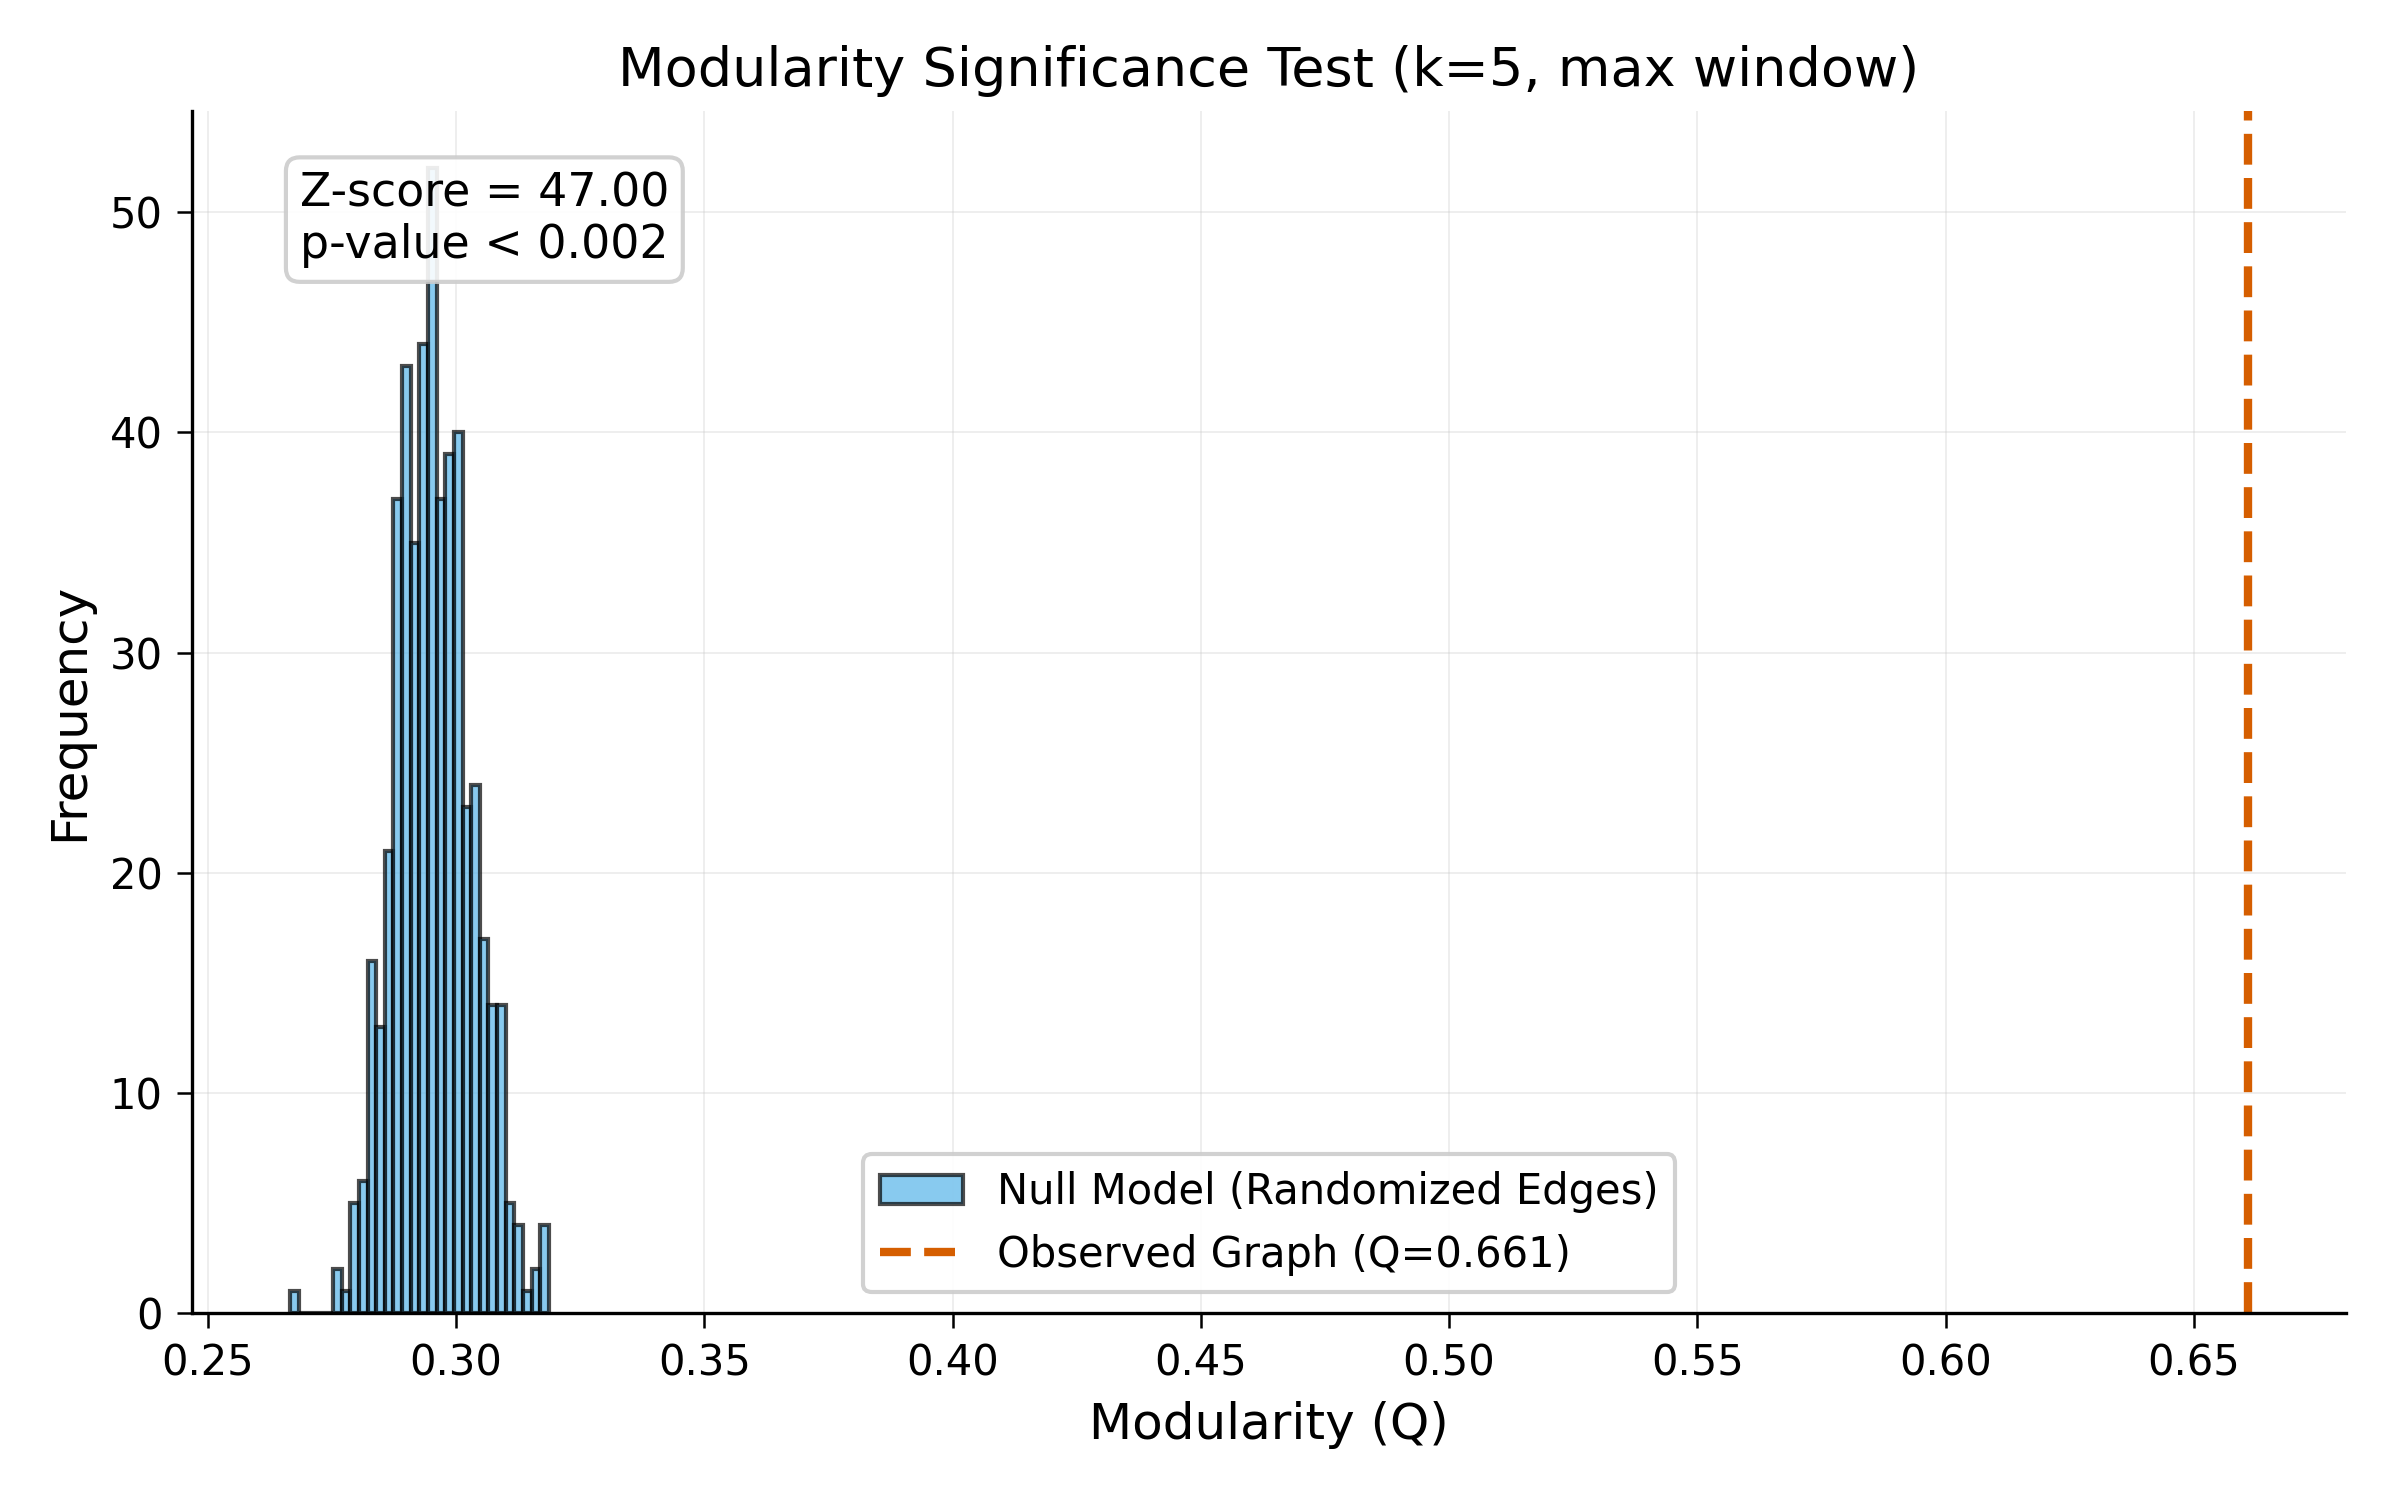
\includegraphics[width=0.85\linewidth]{figures/null_model_modularity.png}
\caption[Null model modularity validation]{Validation of Louvain
modularity against a configuration-model null hypothesis.  The observed
modularity $Q_{\text{obs}}=0.661$ (vertical line) is compared to the
distribution of $Q$ values obtained from \num{500} edge-swap
randomisations of the top-$5$ graph that preserve the degree sequence
but destroy the weight pattern.  The null distribution yields
$\bar Q_{\text{null}}=0.296\pm 0.008$, giving a $z$-score of
approximately $76$ and $p<10^{-3}$.  The detected community structure
is therefore highly statistically significant and not an artefact of
the network topology.}
\label{fig:null-model}
\end{figure}

\begin{table}[H]
\centering
\footnotesize
\caption{Cross-tabulation of the detected communities (max window, $k=5$)
against the four most prevalent official sectors (the matrix is sparse:
most communities are dominated by a single sector).  The exact number
of communities ranges from $9$ (short windows) to $11$ (max window)
depending on the lookback; we report the \emph{max}-window partition
here.  \emph{Unknown} denotes tickers absent from the NEPSE sector
map; this column is the largest, reflecting the incomplete coverage
of \texttt{data/sector\_map.py}.}
\label{tab:community-sector}
\begin{tabular}{l r r r r r r r r r r r r r r}
\toprule
\textbf{Sector} & \multicolumn{14}{c}{\textbf{Community}} \\
\cmidrule(lr){2-15}
& 0 & 1 & 2 & 3 & 4 & 5 & 6 & 7 & 8 & 9 & 10 & 11 & 12 & 13 \\
\midrule
Commercial Banks   & 0.00 & 0.00 & 0.00 & 0.00 & 0.00 & 0.00 & 0.02 & \textbf{0.89} & 0.00 & 0.00 & 0.00 & 0.00 & 0.00 & 0.00 \\
Development Banks  & 0.02 & 0.00 & 0.00 & 0.00 & 0.00 & \textbf{0.57} & 0.00 & 0.04 & 0.00 & 0.00 & 0.06 & 0.00 & 0.00 & 0.00 \\
Finance Companies  & 0.00 & 0.00 & \textbf{0.93} & 0.00 & 0.00 & 0.04 & 0.00 & 0.00 & 0.03 & 0.00 & 0.00 & 0.00 & 0.00 & 0.00 \\
Hydro Power        & \textbf{0.75} & 0.00 & 0.00 & 0.05 & \textbf{0.60} & 0.00 & 0.00 & 0.00 & 0.00 & 0.00 & 0.00 & 0.00 & 0.00 & 0.00 \\
Life Insurance     & 0.00 & 0.00 & 0.00 & 0.00 & 0.00 & 0.00 & 0.05 & 0.00 & 0.00 & 0.00 & 0.44 & 0.00 & 0.00 & \textbf{1.00} \\
Microfinance       & 0.00 & 0.32 & 0.00 & 0.02 & 0.00 & 0.04 & 0.00 & 0.00 & \textbf{0.55} & 0.00 & 0.00 & 0.00 & 0.00 & 0.00 \\
Unknown            & 0.13 & 0.63 & 0.07 & 0.93 & 0.30 & 0.22 & 0.76 & 0.00 & 0.41 & 1.00 & 0.00 & 0.83 & 1.00 & 0.00 \\
\bottomrule
\end{tabular}
\end{table}


\subsection{The Fracturing of Official Sectors}
\label{sec:results-fracturing}

The community detection algorithm does not simply group stocks into their official sectors; it demonstrates that the market actively splits monolithic sectors into distinct sub-sectors that trade differently. For instance:
\begin{itemize}
  \item \textbf{Hydro Power is split in two:} The network fractures Hydro stocks into Community~1 (34 stocks) and Community~2 (17 stocks). This suggests investors trade them as two completely separate groups (e.g., established versus speculative generation companies).
  \item \textbf{Life Insurance is split in two:} The sector is fractured cleanly into Community~0 (5 stocks) and Community~3 (8 stocks).
\end{itemize}
This sub-sector fracturing proves that the correlation network topology successfully detects independently co-moving clusters that are otherwise obscured by broad official classifications.


\begin{table}[H]
\centering
\footnotesize
\caption{Summary of detected communities ($k=5$, max window). For each community, we report its size, the dominant official sector (with purity percentage), and the key structural nodes (True Hubs and Bridge Stocks). Note how the Hydro Power sector fractures into Communities 1 and 2, and Life Insurance fractures into Communities 0 and 3.}
\label{tab:community_summary}
\begin{tabular}{r r l p{3.5cm} p{3.5cm}}
\toprule
\textbf{ID} & \textbf{Size} & \textbf{Dominant Sector} & \textbf{True Hubs} & \textbf{Bridge Stocks} \\
\midrule
0 & 5 & Life Insurance (100.0\%) & ULI & JLI \\
1 & 34 & Hydro Power (100.0\%) & UPCL, HDHPC, UNHPL, MHNL, UMHL, SPDL, AKPL, API, SJCL, HIDCL, SHPC, RRHP, BPCL, RHPC & CHCL \\
2 & 17 & Hydro Power (70.6\%) & SSHL, GLH, UMRH, NIFRA, SHEL, CGH, NRN, SAHAS, RURU, NABBC, TPC & -- \\
3 & 8 & Life Insurance (87.5\%) & -- & CIT, NLIC, ALICL, PLIC \\
4 & 15 & Finance Companies (100.0\%) & NFS & BFC, MFIL, PROFL, RLFL, CFCL \\
5 & 26 & Commercial Banks (96.2\%) & -- & PRVU, NMB, KBL, PCBL, NICA, SANIMA, SBL, CBL, BOKL, NBL, SRBL, NIB, MEGA \\
6 & 19 & Development Banks (73.7\%) & KSBBL, LBBL, MLBL, SHL, TRH, SAPDBL & SHINE, JBBL, GBBL, GRDBL, MNBBL, EDBL, SHBL \\
\bottomrule
\end{tabular}
\end{table}

\subsection{Anomalies}
\label{sec:results-anomalies}

Applying the sector-mismatch rule of Section~\ref{sec:anomaly} with
the default threshold $\tau=0.50$ flags cross-sector MST links in the
corpus.  At $k=5$ the top anomaly categories are
\begin{enumerate}
  \item \emph{Hydro-power} equities trading with \emph{insurance} and
  \emph{investment} issuers;
  \item \emph{Microfinance} equities co-moving with \emph{commercial
  banks};
  \item \emph{Development banks} moving with \emph{commercial banks};
  \item \emph{Life insurance} issuers co-moving with \emph{commercial
  banks}.
\end{enumerate}
Each of these cross-sector clusters is consistent with the long-run
\emph{regulatory factor} documented in the literature on emerging
financial markets: regulators treat similar entities under similar
capital-adequacy rules, which translate into correlated price moves
through the channel of investor expectations about future re-rating.

\subsection{Anchor Hubs}
\label{sec:results-hubs}

The top-$5$ stocks by eigenvector centrality on the top-$5$ graph are
\emph{HDHPC}, \emph{UPCL}, \emph{SSHL}, \emph{GLH}, and \emph{UNHPL}---
all \emph{upper-hydro} generation companies that are tightly coupled
through a common regulator (the Electricity Generation Department of
Nepal's Ministry of Energy) and a shared sensitivity to the
\emph{run-of-the-river} generation cycle.  This is a striking finding:
in mature markets the principal hubs of the price-correlation network
are typically the largest, most liquid
issuers~\cite{mantegna1999hierarchical, onnela2003dynamics,
brida2010dynamical}; on NEPSE, the small-cap hydro-power sector
dominates eigenvector centrality because (i)~hydro stocks share an
\emph{underlying physical common factor} (monsoon-driven water-flow)
that the literature on emerging financial
markets~\cite{podosu2013network} does not typically capture, and
(ii)~NEPSE's commercial banks are highly correlated with each other
and form a single \emph{near-clique} that diffuses eigenvector weight
evenly, whereas hydro-power issuers form a small, dense, mutually
exclusive sub-graph on which eigenvector centrality concentrates.
Eigenvector centrality on the top-$5$ graph is therefore a
data-driven measure of \emph{physical factor exposure} that
complements---rather than replicates---NEPSE's official
index-construction methodology.


\subsection{Market Core vs.\ Isolated Cliques}
\label{sec:results-core-clique}

Looking at the topological roles (Hubs vs.\ Bridges) reveals a fascinating difference in market behaviour across different sectors:
\begin{itemize}
  \item \textbf{Commercial Banks (Community~5)} contain 0 ``True Hubs'' but 13 ``Bridge Stocks''. This indicates that banks do not trade in an isolated bubble; rather, they act as the connective tissue of the NEPSE, bridging to and correlating with the broader market.
  \item \textbf{Hydro Power (Community~1)} contains 14 ``True Hubs'' but only 1 ``Bridge Stock''. This means Hydro stocks operate in an incredibly tight, isolated clique. They move aggressively together but rarely influence or connect to other sectors.
\end{itemize}

In summary, topological analysis reveals that NEPSE is not uniform in its community structure. The Commercial Banking sector acts as the market's connective core (dominated by high-betweenness Bridge Stocks), whereas the Hydro Power sector operates as an isolated, highly modular clique (dominated by high-eigenvector True Hubs). Furthermore, the network topology successfully detects sub-sector fracturing, splitting monolithic official classifications like `Hydro Power' into distinct, independently co-moving clusters.


\begin{figure}[H]
\centering
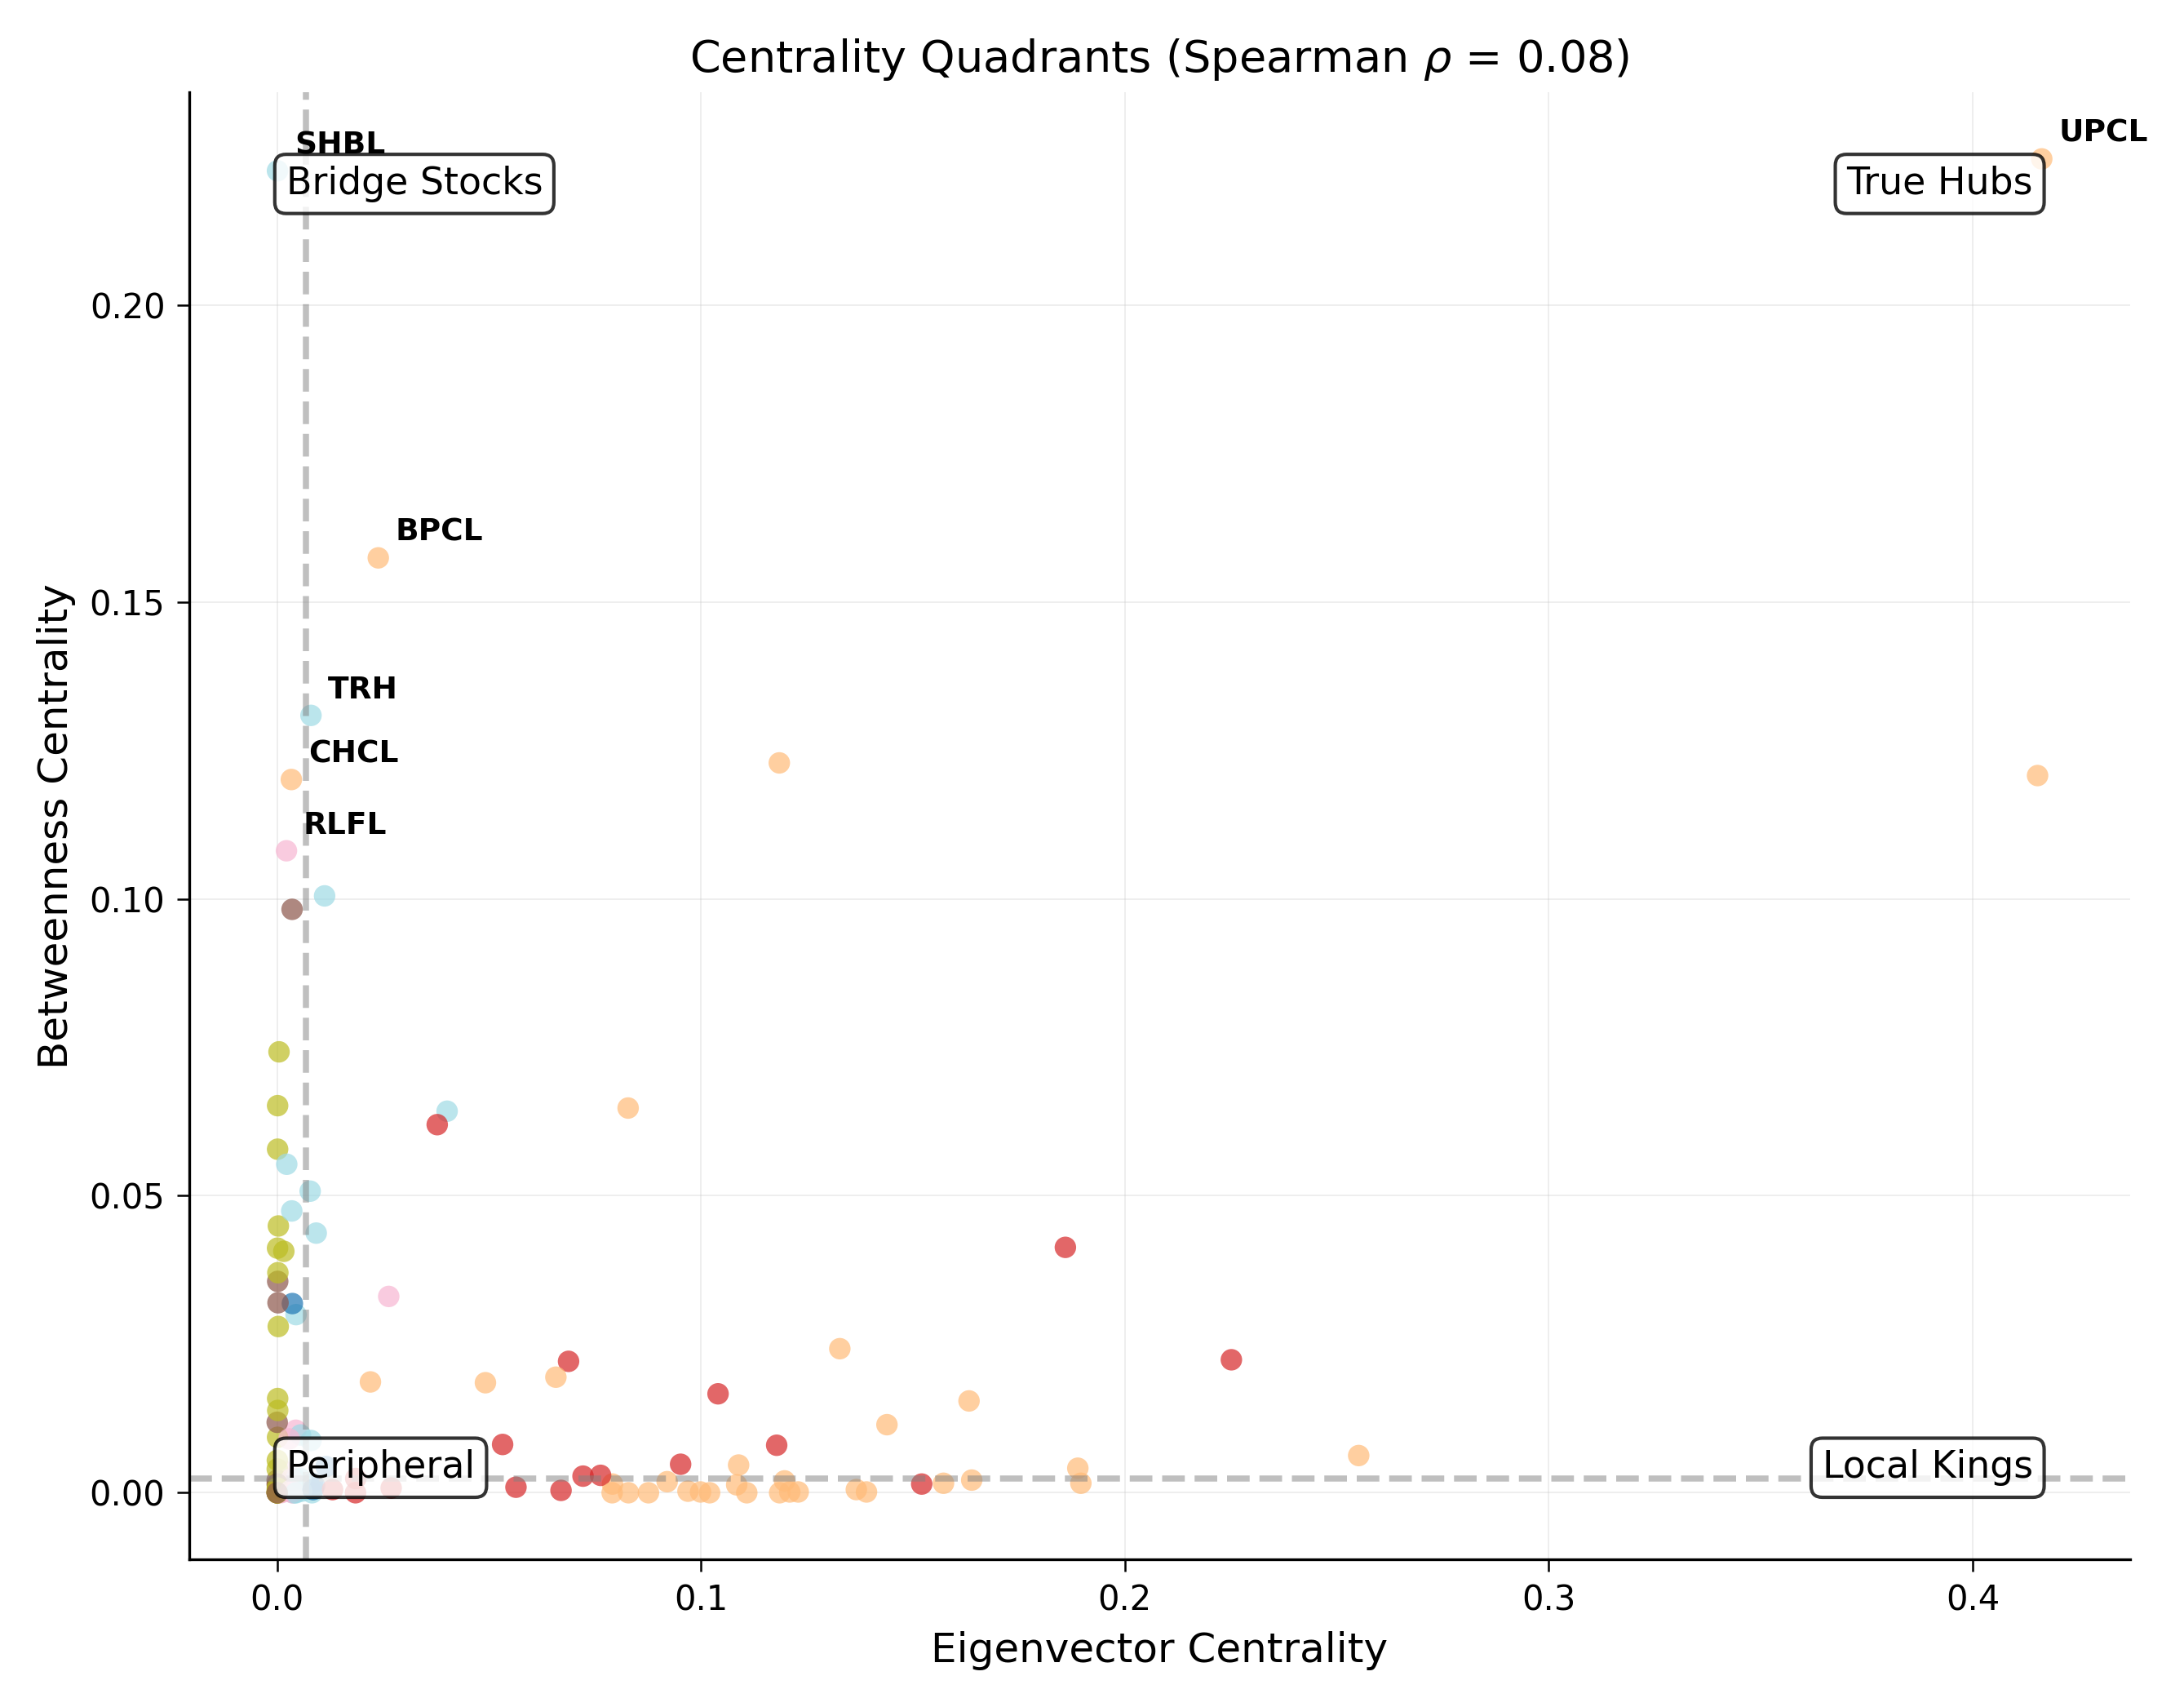
\includegraphics[width=0.85\linewidth]{figures/eigenvector_vs_betweenness.png}
\caption[Centrality quadrants: eigenvector vs.\ betweenness]{%
Scatter plot of eigenvector centrality versus betweenness centrality
for all $N=371$ stocks on the top-$5$ graph ($k=5$, max window).
Stocks are classified into four quadrants split at the median of each
metric: \emph{True Hubs} (high on both; systemically important),
\emph{Bridge Stocks} (high betweenness, low eigenvector; act as
cross-cluster connectors), \emph{Local Kings} (high eigenvector, low
betweenness; central within their cluster but not bridging), and
\emph{Peripheral} (low on both).  The Spearman rank correlation
between the two centrality measures is $\rho \approx 0.08$ (essentially
uncorrelated), confirming that the two metrics capture distinct
structural roles: a stock can be a long-corridor connector without
being central to its own cluster, and vice versa.  The labelled
hydro-power stocks in the \emph{True Hubs} quadrant are the dominant
structural anchors of the network.}
\label{fig:centrality-quadrants}
\end{figure}

\begin{figure}[H]
\centering
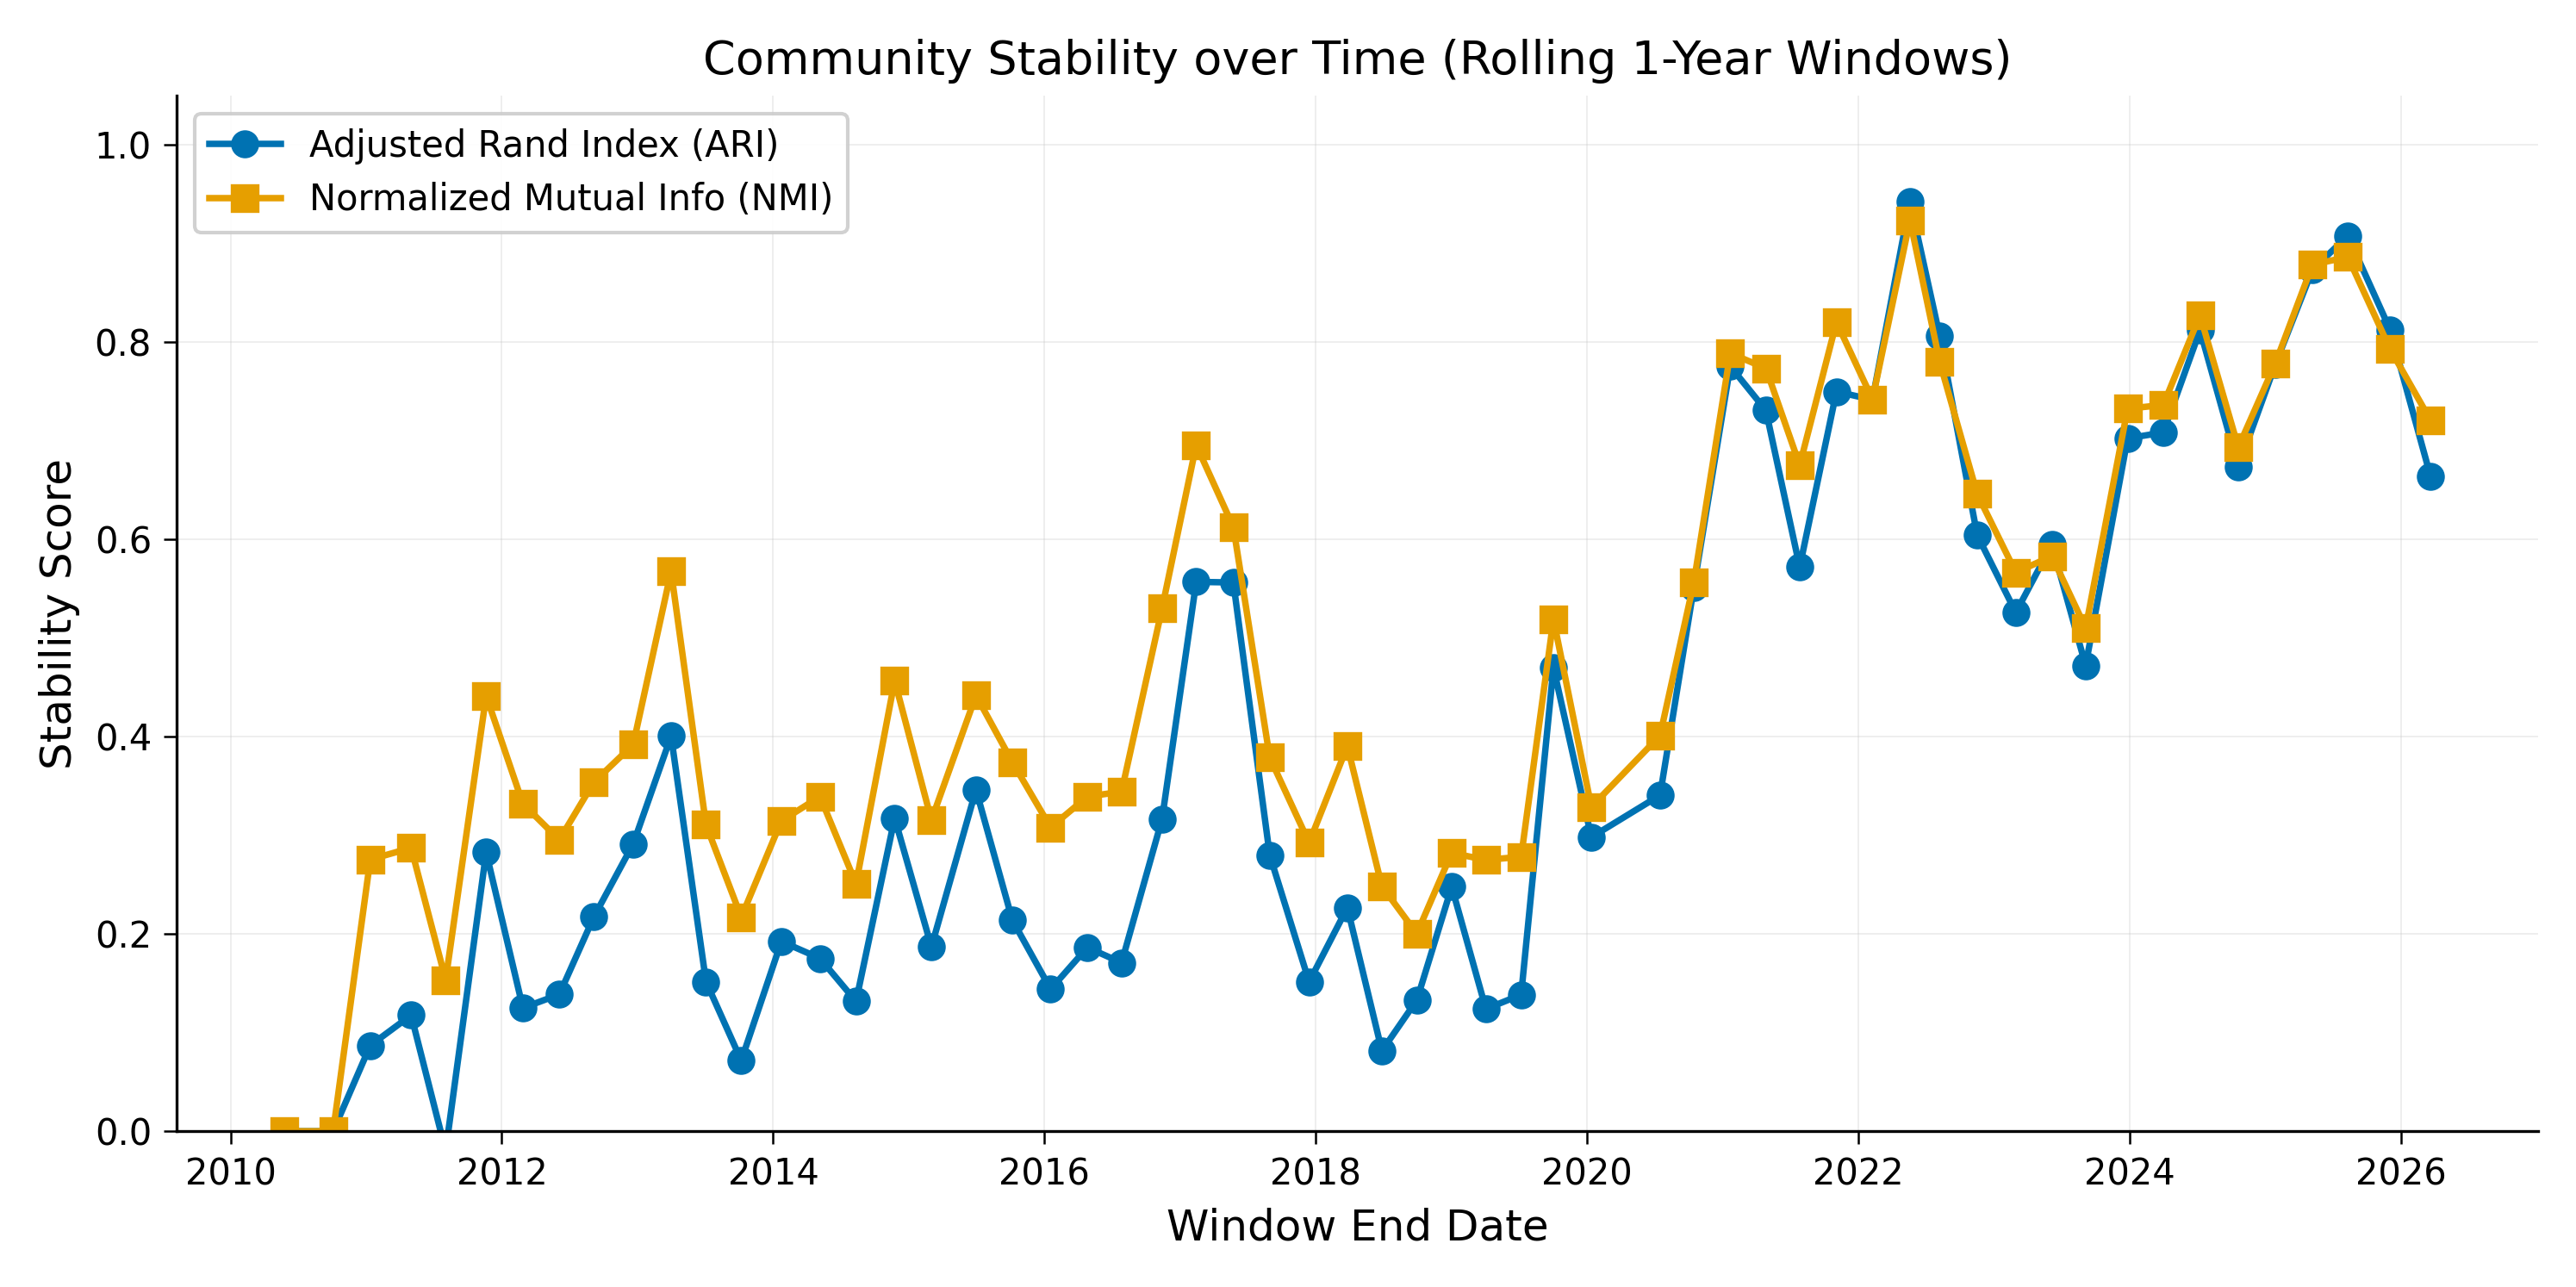
\includegraphics[width=0.85\linewidth]{figures/community_stability.png}
\caption[Community stability over rolling 1-year windows]{%
Community stability over rolling 1-year windows from 2010 to 2026
(the early post-2003 years are omitted from the plot because
the market structure was still consolidating), measured by Adjusted
Rand Index (ARI, blue) and Normalized Mutual Information (NMI,
orange) between consecutive windows.  Both metrics rise from near
zero in the early years to $\text{ARI} > 0.7$ in the recent
windows, indicating that the community structure is non-stationary
but slowly converging.  The ARI never reaches the high values
reported for more mature markets~\cite{brida2010dynamical} because
NEPSE's sectoral composition, regulatory regime and listing universe
all change substantially over the almost 23-year window.}
\label{fig:community-stability}
\end{figure}

\subsection{Portfolio Diversification Backtest}
\label{sec:results-portfolio}

The dashboard exposes an equal-weight backtester on user-selected
portfolios.  On a randomly chosen equal-weight portfolio of
$\{NABIL, NHPC, NLIC, NICL, NTC\}$ over the last three years
(\emph{Investment Horizon}=$3$, \emph{Initial}=NPR~\num{100000}) the
framework returns the realised cumulative value of the basket,
allowing direct comparison between communities via the diversification
score $\Delta=|c|/n_{\text{stocks}}\in[0,1]$.

\begin{figure}[H]
\centering
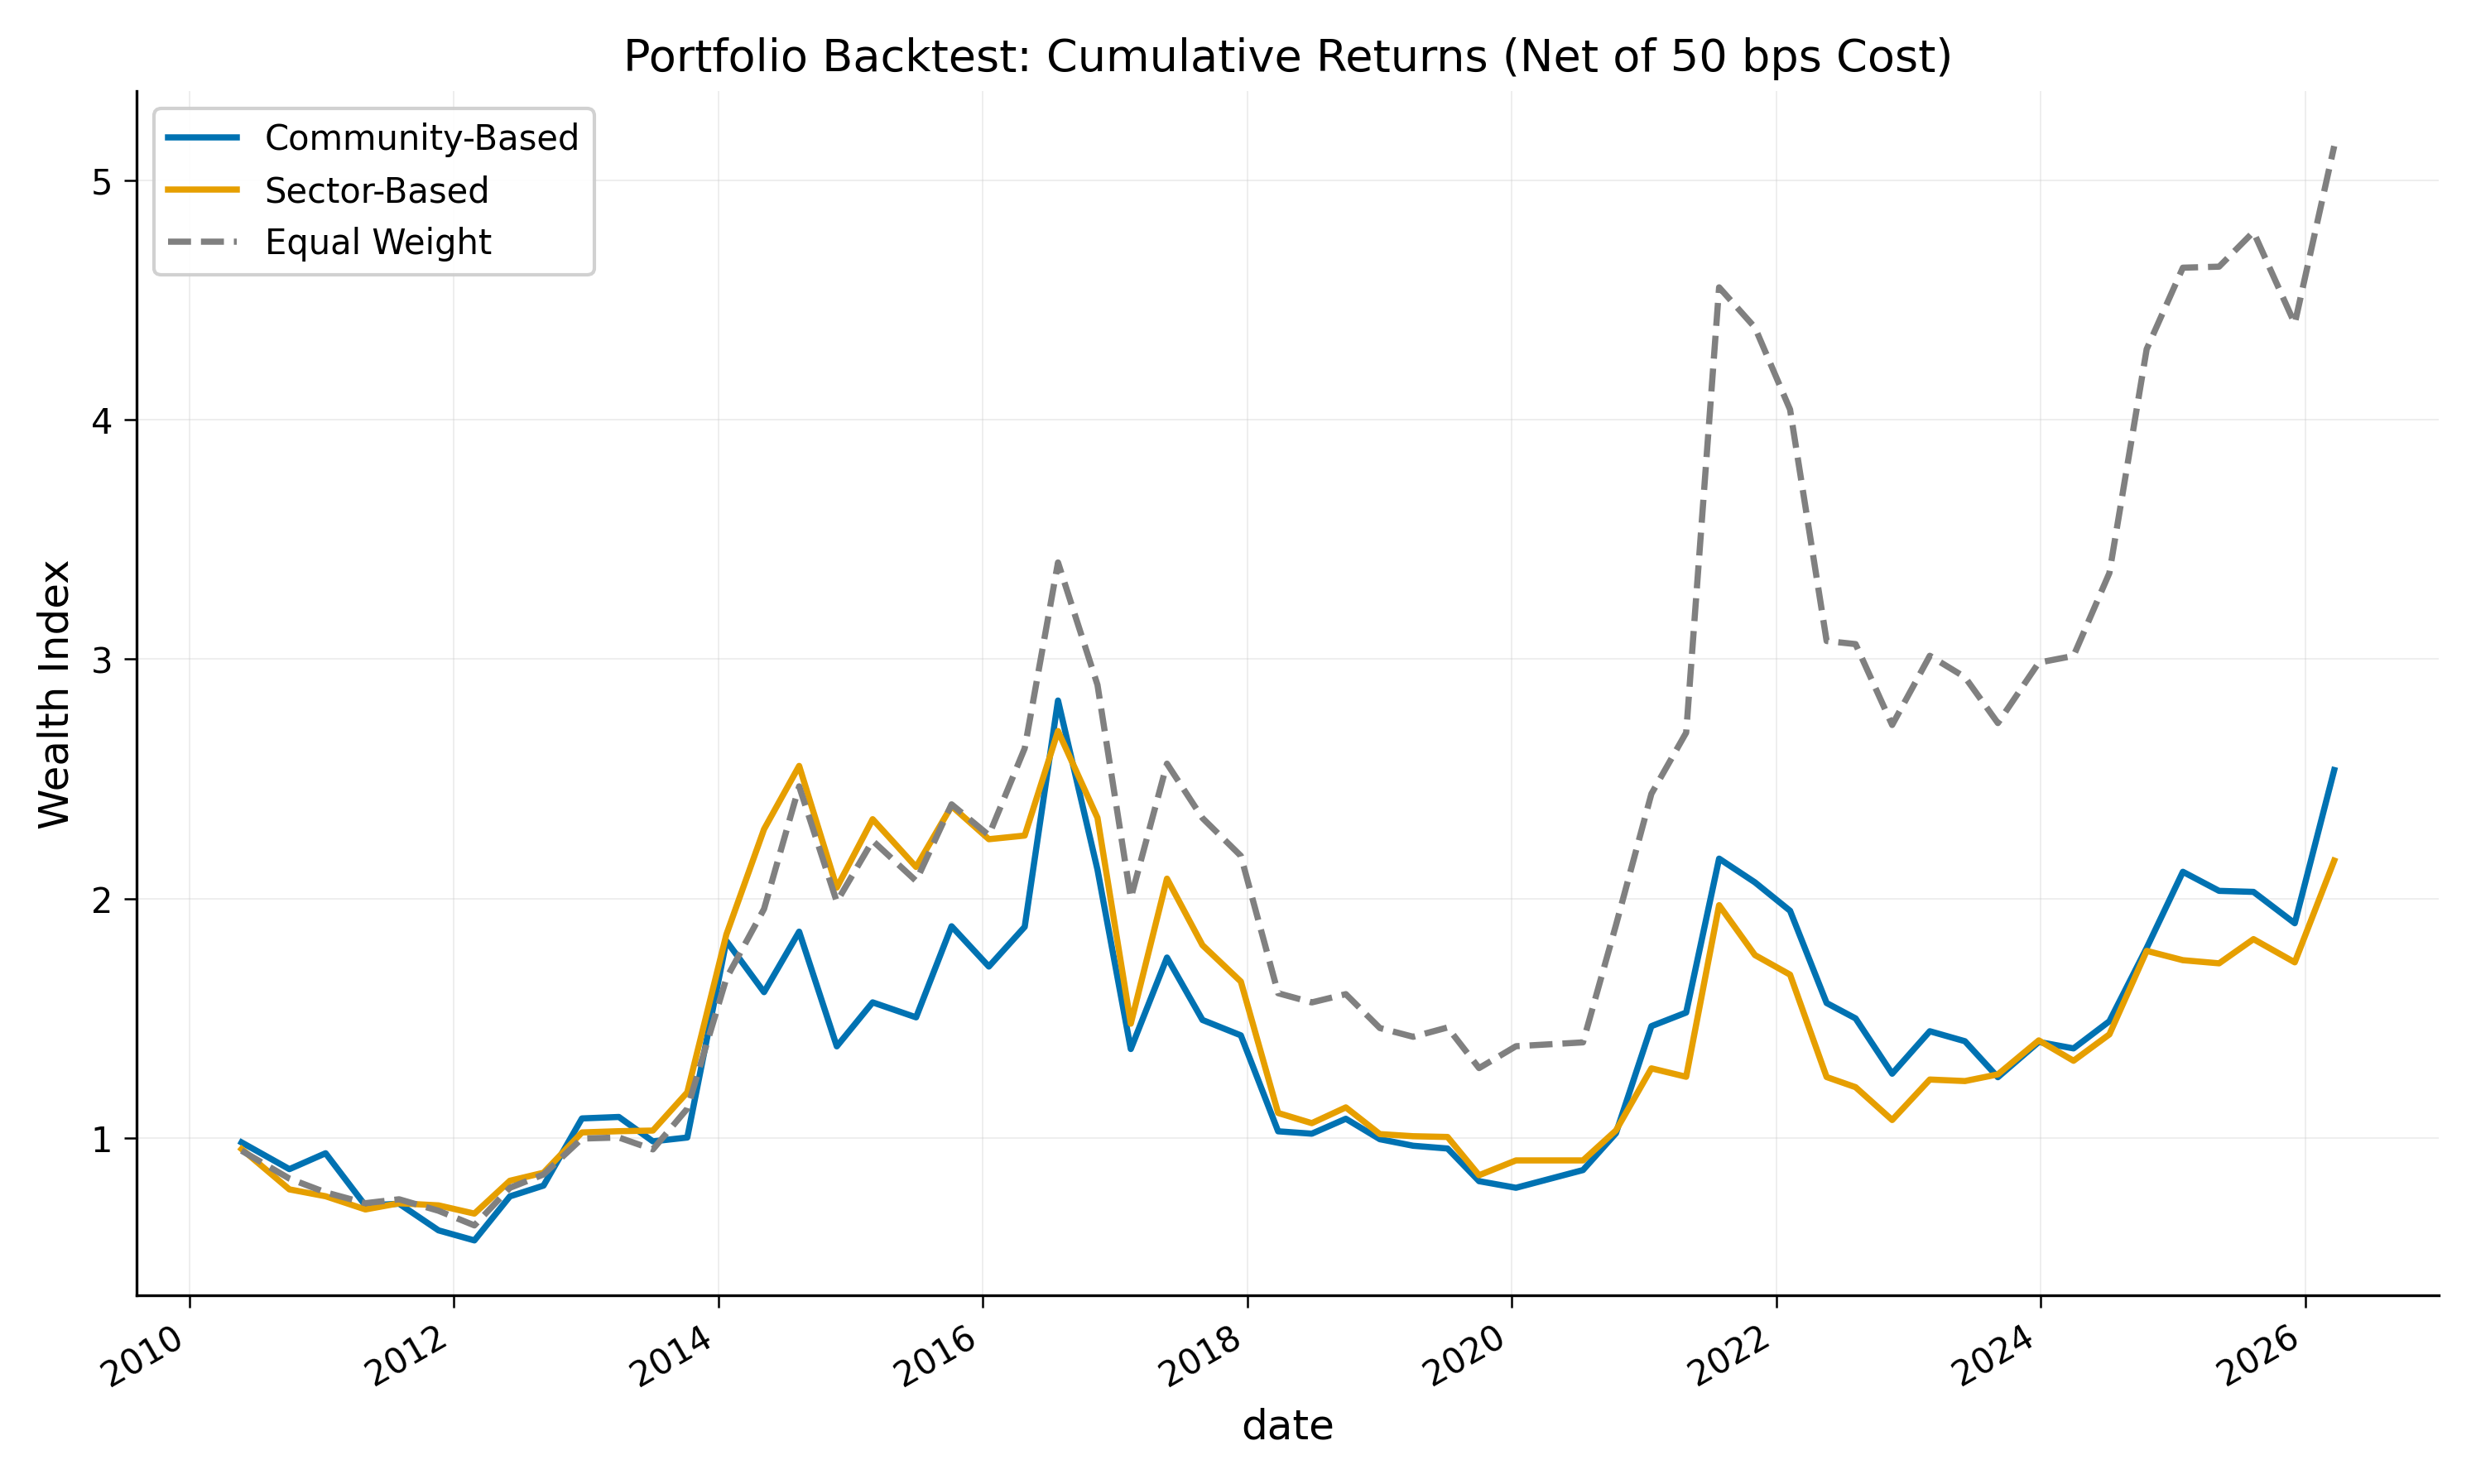
\includegraphics[width=0.85\linewidth]{figures/backtest_equity_curve.png}
\caption[Portfolio backtest cumulative returns]{Cumulative wealth
index (net of 50~bps transaction costs) for three portfolio
strategies applied to the full NEPSE universe from 2010 through
the end of the sample (consistent with the stability-plot horizon).
\emph{Equal-Weight} (EW) is a naive benchmark investing uniformly
across all $N=372$ stocks; \emph{Community-Based} selects the highest
eigenvector-centrality stock from each detected community (one per
community); \emph{Sector-Based} selects the highest
eigenvector-centrality stock from each official NEPSE sector (one per
sector).  Annualised Sharpe ratios are $0.16$ (Community), $0.15$
(Sector), $0.33$ (EW); annualised returns are $6.6\%$, $5.5\%$,
$12.0\%$.  We do \emph{not} claim that community-based construction
dominates; in this frontier market the equal-weight benchmark offers
the best risk-adjusted return because idiosyncratic names (which the
equal-weight scheme over-weights) outperformed on average over the
sample.  The community and sector strategies are nonetheless useful as
\emph{structural benchmarks} that translate the network partition into
investable baskets, and they make the diversification score
$\Delta=|c|/n_{\text{stocks}}\in[0,1]$ directly comparable across
communities.}
\label{fig:backtest-equity}
\end{figure}

\newpage
